\section{Kanalcodierung}
\subsection{CRC}
\subsubsection{CRC-Polynomdivision}
\begin{itemize}
    \item Nutzdatenwort: $111010100$
    \item Generatorpolynom: $x^3 + x^2 + 1 \Rightarrow$ $\textcolor{blue}{1101}$
    \item Nutzdatenwort mit Nullen (Grad des Generatorpolynoms [3]) erweitern: $111010100\textcolor{red}{000}$
    \item Rest bestimmen durch Division: $100$
    \item Rest an Nutzdatenwort anhängen: $111010100\textcolor{red}{100}$
\end{itemize}
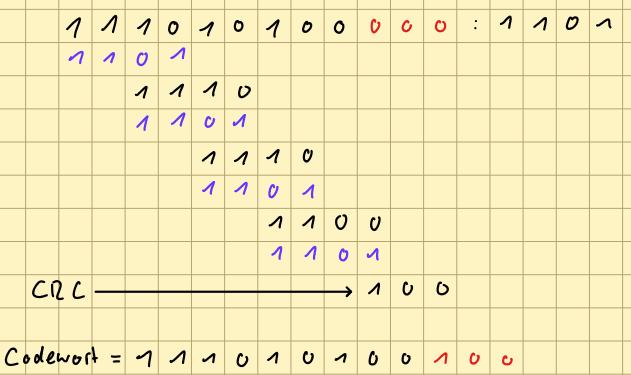
\includegraphics[scale=0.55]{crc_div}
